\documentclass[a4paper, 12pt]{article}
\usepackage[hmargin=2cm,vmargin=2.5cm]{geometry}
\usepackage[italian]{babel}


\usepackage{enumerate}
\usepackage{makecell}
\usepackage{graphicx}
\usepackage{hyperref}
\usepackage{amsmath}
\usepackage[backend=biber,style=apa, url=true, sortcites]{biblatex}
\usepackage[table]{xcolor}
\usepackage{minted}
\usepackage{graphicx}


\addbibresource{references.bib}
\hypersetup{
    colorlinks,
    citecolor=black,
    filecolor=black,
    linkcolor=black,
    urlcolor=black
}

\setlength{\arrayrulewidth}{0.4mm}

\newcommand{\HRule}{\rule{\linewidth}{0.5mm}}

\begin{document}
\selectlanguage{italian} 

\begin{titlepage}
  \begin{center}
    % logo
    
\includegraphics[width=0.5\textwidth]{main/figures/logo.png}~\\[1cm]

    \vspace{3cm}

    \textsc{\Large Complementi di Matematica: \\ EDO e loro applicazioni}\\[3cm]


    \HRule \\[0.4cm]
    {\large \bfseries Studio analitico di un sistema di oscillatori attraverso le EDO \\ e sistemi numerici per risoluzione numerica \\ [0.4cm]}
    \HRule \\[4cm]

    \large\textbf{Studenti:}\\
    Cairone Giuseppe \\ Rossi Gianmarco \\ Scuola Superiore di Studi Universitari \\ e di Perfezionamento Sant'Anna\\[3cm]

    \vfill

    {\large 20/13/2023}

  \end{center}
\end{titlepage}

\newpage

\tableofcontents

\newpage

\section{Introduzione}

Per questo progetto si intende studiare un sistema composto da $n$ pendoli, ciascuno con massa $m$ e braccio di lunghezza $l$ (non massivo), fissati ad un supporto di massa $M$.

\begin{figure}[htp!]
  \centering
  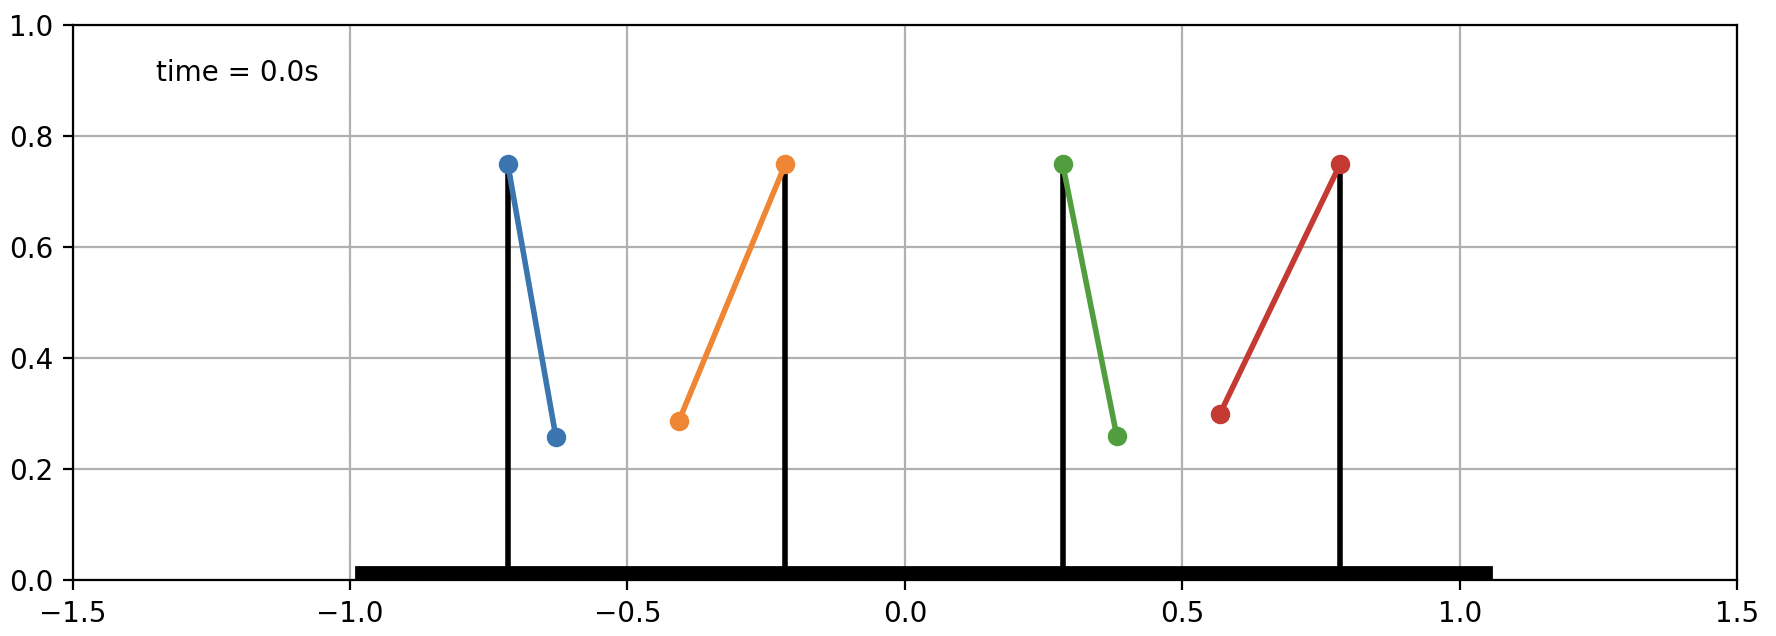
\includegraphics[width=.7\textwidth]{main/figures/fig_pendoli.png}
  \caption{Condizione iniziale per 4 pendoli}
  \label{fig:pendoli_start}
\end{figure}

Il sistema ha quindi $n + 1$ gradi di libertà, uno legato al moto orizzontale del supporto e uno per ogni pendolo. Il primo è determinato dalla posizione $x(t)$ del supporto, i gradi di libertà associati ai pendoli sono determinati dall'angolo del pendolo rispetto alla verticale $\theta_i(t)$. Per ciò che si è interessati a studiare poniamo $x(0) = 0$, $\dot{x}(0) = 0$. Dunque lo stato iniziale è determinato da $\theta_i(0), \dot{\theta_i}(0)$ per ogni $i$-esimo pendolo con $1 \le i \le n$.

\section{Oscillazioni libere}

Per studiare il sistema si fa uso delle equazioni di Eulero-Lagrange, le quali ci permettono, a partire dall'energia cinetica e quella potenziale, di ricavare le equazioni del moto per il sistema.

\subsection{Energia del Sistema}

Si parte quindi andando a scrivere le equazioni per ricavare l'energia cinetica del sistema che risulta essere
\[
K = \frac{1}{2} M \dot{x}^2 + \frac{1}{2} \sum_{i = 0}^n m v_i^2
\]
dove le varie $v_i$ sono le velocità delle masse nel sistema di riferimento del laboratorio quindi:
\[
v_i^2 =\left( l \dot{\theta_i} \sin \theta_i \right) ^ 2 + \left( \dot{x} + l \dot{\theta_i} \cos \theta_i \right) ^ 2
\]
L'energia potenziale la calcoliamo ponendo lo zero del potenziale nel vertice di oscillazione dei pendoli in modo da semplificare l'espressione della stessa e quindi anche i calcoli. In definitiva si ottiene che: 
\[
U = - \sum_{i = 0}^n mgl\cos \theta_i
\]

Da notare che non viene considerata l'energia potenziale del supporto  perché rimane costante nel tempo. Interessando a noi la differenza di energia potenziale tutti i termini costanti possono quindi essere omessi.

\subsection{Lagrangiana del Sistema}

Una volta scritte le equazioni delle energie possiamo procedere a scirvere la lagrangiana del sistema ovvero:
\[
L\left(x, \dot{x}, \theta_i, \dot{\theta_i}\right) = K - U = \frac{1}{2} M \dot{x}^2 + \frac{1}{2} \sum_{i = 0}^n m v_i^2 + \sum_{i = 0}^n mgl\cos \theta_i
\]

Per ottenere il sistema di equazioni differenziali del moto 
applico l'equazione di Eulero-Lagrange ad ogni coordinata
% \[
% \frac{{\partial L}}{{\partial q}} - \frac{{d}}{{dt}}\left(\frac{{\partial L}}
% {{\partial \dot{q}}}\right) = 0 
% \]

\[
\frac{{\partial L}}{{\partial q_j}}\left(\textbf{q}, \dot{\textbf{q}}, t\right) - \frac{{d}}{{dt}} \frac{{\partial L}}
{{\partial \dot{q_j}}}\left(\textbf{q}, \dot{\textbf{q}}, t\right) = 0 
\]

Si ottiene quindi il sistema
% \begin{align*}
% \begin{aligned}
\[
\begin{cases}
     \dfrac{\partial L}{\partial \theta_1} =& \dfrac{d}{dt}\dfrac{\partial L}{\partial \dot{\theta_1}} \\
     \vspace{.3cm}
    \ldots \\
    \vspace{.3cm}
    \dfrac{\partial L}{\partial \theta_n} =& \dfrac{d}{dt}\dfrac{\partial L}{\partial \dot{\theta_n}} \\
    \vspace{.3cm}
    \dfrac{\partial L}{\partial x} =& \dfrac{d}{dt}\dfrac{\partial L}{\partial \dot{x}} \\
\end{cases}
% \end{aligned}
\quad \Rightarrow \quad
% \begin{align*}
\begin{cases}
    \ddot{\theta}_1 = \dfrac{gsin(\theta_1)-\ddot{x}cos(\theta_1)}{l} \\
    \vspace{.3cm}
    \ldots \\
    \vspace{.3cm}
    \ddot{\theta}_n = \dfrac{gsin(\theta_n)-\ddot{x}cos(\theta_n)}{l} \\
    \vspace{.3cm}
    % \ddot{x} =& \dfrac{ml\sum_{i=1}^{n} \dot{\theta_i^2 } \sin(\theta_i) -mg\sum_{i=1}^{n} \sin(2 \theta_i)}{M+m\sum_{i=1}^{n}sin^2(\theta_i)} \\
    \ddot{x} = \sum_{i=1}^{n}  \frac{ml \dot{\theta_i^2 } \sin(\theta_i) -mg \sin (2 \theta_i)}{M+m \sin^2(\theta_i)} \\
    \sum
\end{cases}
\]
% \end{align*}

Andando a risolvere per le coordinate $x(t)$ e $\theta_i(t)$ si ottiene l'evoluzione del sistema

\section{Risoluzione numerica}

Una volta analizzato analiticamente il sistema dinamico si procede a risolvere le equazioni. Dato che non esiste una funzione esplicita che risolva le equazioni differenziali ottenute. Si usa quindi un sistema numerico per ottenere un risultato.

\subsection{Metodo numerico}

Per risolvere numericamente le equazioni differenziali abbiamo scelto di usare il metodo numerico di Runge-Kutta di ordine 4. Questo metodo garantisce la simpletticità del sistema ovvero che l'energia totale del sistema rimanga quanto più costante e limitata nel tempo. Proprio quest'ultimo fattore è importante in quanto il sistema iniziale prevede una conservazione dell'energia totale, aspetto che deve rispecchiarsi anche nel metodo numerico.

\subsection{Implementazione}



\begingroup
\obeylines
\inputminted[fontsize=\scriptsize, linenos, breaklines=true, xleftmargin=0.75cm, frame=lines]{cython}{code/Python/file_1.pyx}
\endgroup

\newpage

\end{document}